%%%%%%%%%%%%%%%%%%%%%%%%%%%%%%%%%%%%%%%%
% introduction

Shape is one fundamental object property used in several robotic tasks \citep{Bajcsy1989Machine}. It is the task that determines the exact nature of the best representation of shape, but there are several desirable features in general: accuracy, conciseness, intuitive parametrization, local support, affine invariance, arbitrary topology, guaranteed continuity, efficient rendering and efficient intersections, among others. There are some that are not really special for most robotic tasks such as intuitive parametrization or conciseness. Since we are dealing with arbitrary novel objects, the capacity to represent arbitrary topologies with guaranteed continuity is desirable. Implicitly defined surfaces have these properties. There are several ways to define an implicitly defined surface, e.g. via algebraic equations, blobby models and variational surfaces. These classical specifications do not consider any uncertainty measure though. There is where the work by \citet{Williams2007Gaussian} comes in, introducing the notion of a Gaussian Process implicit surface (GPIS). This might not be the only representation to account for uncertainty, but it meets the requirements for a good shape representation in robotic contexts, as has been shown in the discussion of related work. Subsection~\ref{sec:gpis} introduces the notation for GPIS.

Such a representation considers the estimated surface to be the mean value of a Gaussian Process, that is the $0$-level of an implicitly defined manifold. \citet{Henderson1993COMPUTING} provides a way to compute implicitly defined surfaces via continuation techniques. That work has evolved in different manners for different purposes, including one that is of particular interest for our approach: the AtlasRRT algorithm, a path planning method for constrained mechanisms by \citet{Jaillet2013Path}. This combines continuation techniques with Rapidly-exploring Random Trees (RRT) \citep{LaValle2011Motion}, to allow the computation of paths in a constrained configuration space, i.e. a manifold embedded in an ambient space. However, as presented, there is no notion of uncertainty of the manifold itself---recall, this is the object surface in our case. By combining the AtlasRRT algorithm with the concept of GPIS we can derive a powerful planner for traversing an uncertain surface. Subsection~\ref{sec:atlas-rrt} describes the basic idea behind the AtlasRRT algorithm.

The last, but not least, ingredient is the equipment necessary to simulataneously grasp an object with one hand whilst exploring it with another. In Subsection~\ref{sec:scope}, we enumerate considerations for the hardware that is to execute tactile exploration, as well as possible limitations. Finally, with all these ingredients in mind, we formally define the problem we aim to solve in the last subsection.

%Active perception enables a robot to reason on how to efficiently acquire more (task-related) information in a noisy environment in order to complete a task at hand.
%The task we pursue in this work is to enable a robot to reason on how to autonomously combine visual and haptic information to identify the shape of household objects that can be successively grasped and manipulated by a human-sized hand.

%Our approach is to formalise the problem of shape representation as a problem of linear regression, in which a Gaussian Process (GP) is employed to learn a probabilistic model of the object. The GP allows us to build a \emph{maximum a posteriori} (MAP) estimation of the object's surface described as an implicit function, $f(\mathbf{x})=0$, (the 0-levelset of the approximating function) as well as to constrain the learnt function on visual and haptic clues in order to converge to the real shape of the object. To enable the robot to select best-next (exploration) actions, we construe the function $f(\mathbf{x})$ as a manifold and we grow an exploration tree, similar to the AtlasRRT described in~\cite{Jaillet2013Path}, which is biased to visit uncertain region of the object's surface.

%This section proceeds as follows. We firstly introduce the general formulation for GPR for implicit surfaces. We then show how to compute first-order quantities from the GP (surface normals) which are essential to locally parametrise a manifold (Atlas). Finally, we present how to build a sample-based exploration on the manifold to visit regions of the object's surface that are more promising to reduce the global model uncertainty.

%\todo[]{Equipment specification and assumptions have been removed. They should be move later when describing the experimental setup.}
% CR the idea is the you specified abstractly what are the hardware requirements this algorithm is supposed to work with, and then in the experiment you say what hardware you use that comply with the requirements


%%%%%%%%%%%%%%%%%%%%%%%%%%%%%%%%%%%%%%%%
%\subsection{Background}
%\label{sec:resources}

%---------------------------------------
\subsection{Gaussian Process Implicit Surfaces}
\label{sec:gpis}
\begin{figure}[thb]
    \centering
    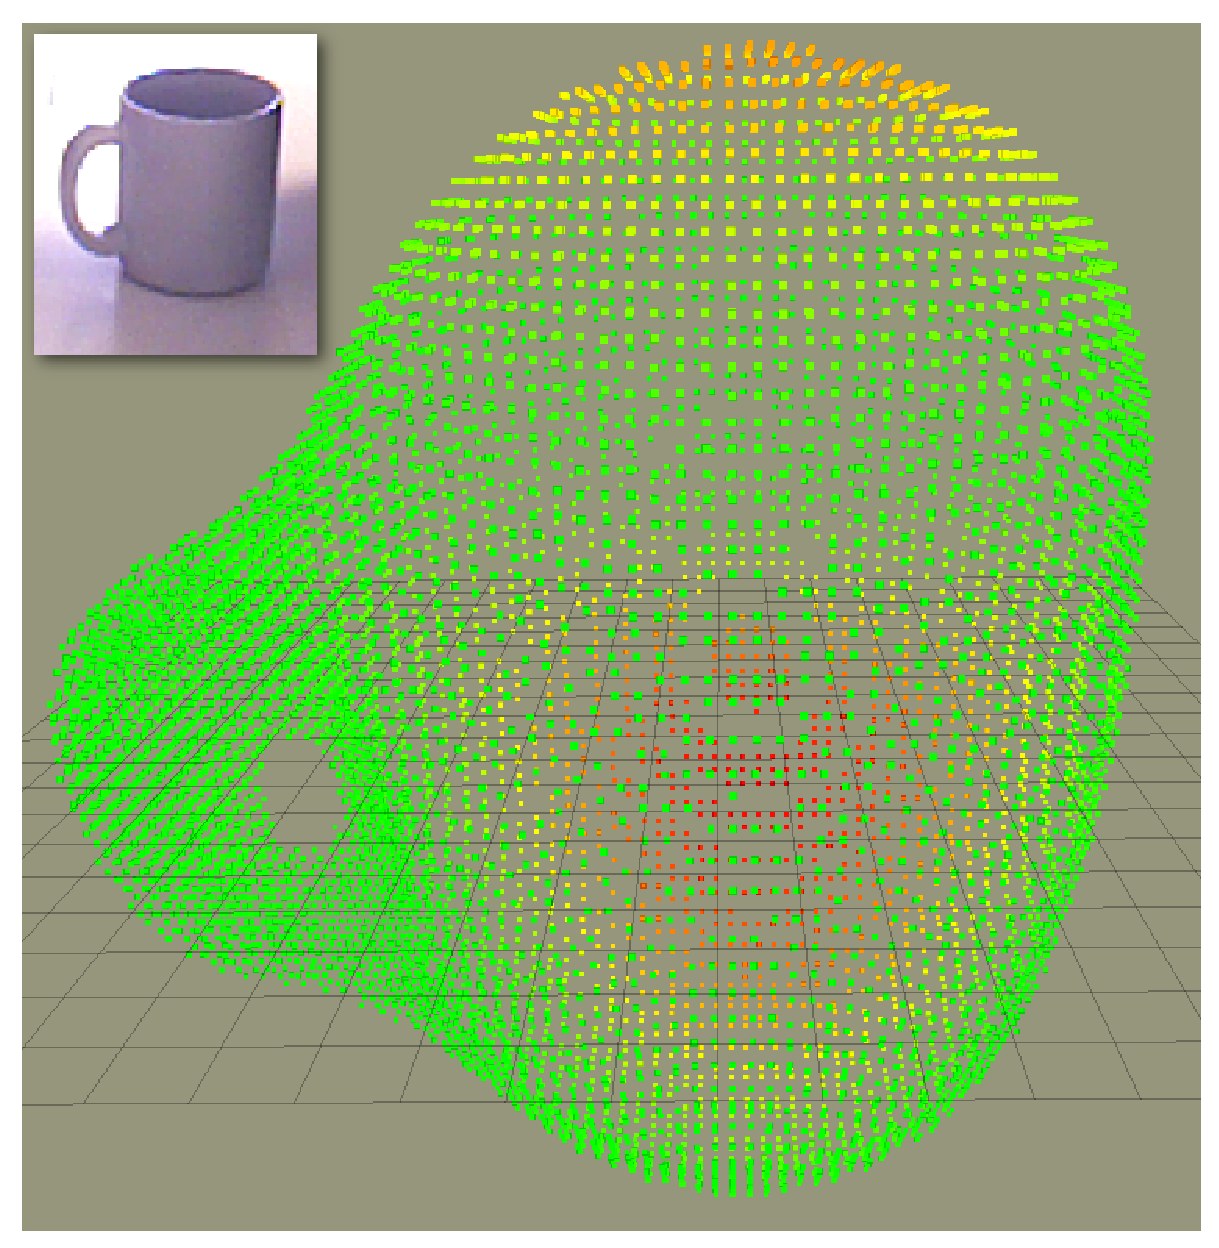
\includegraphics[width=0.95\columnwidth]{mugS.eps}
    \caption{Gaussian Implicit Surface, obtained from a mug (top-left corner) and sampled with a box-grid evaluation with fairly high point density. Each point has a predicted target $y_* \sim= 0$ and is colored accordingly to its associated
    predicted variance, from red (high variance) to green (low variance).}
    \label{fig:gpmug}
\end{figure}

A surface in 3D can be regarded as the $0$-level set of a family of surfaces defined by an implicit function $F(\mathbf{x}, y)=0$, where $F:\mathbb{R}^{3+1}\rightarrow \mathbb{R}$, with coordinates $\mathbf{x}\in \mathbb{R}^3$ and parameter $y\in \mathbb{R}$.
 Under the assumption that the Implicit Function Theorem holds, it can be expressed, at least locally, as $y = f(\mathbf{x})$, with $F(\mathbf{x},f(\mathbf{x}))=0$, and the surface of our interest raises when setting $y = 0$ --- the $0$-level set. Naturally, the value of $f$ (or $y$) increases to a positive value in outward normal direction to the surface ($\nabla F$), and decreases to a negative value in the inward direction ($-\nabla F$).

A Gaussian process (GP), on the other hand, ``is a collection of random variables, any finite number of which have a joint Gaussian distribution'' \citep[Def. 2.1]{Rasmussen2006Gaussian}, and it is completely specified by a mean, $m(\mathbf{x}) = \mathbb{E}[f(\mathbf{x})]$, and a covariance, $k(\mathbf{x},\mathbf{x}') = \mathbb{E}[(f(\mathbf{x}) - m(\mathbf{x}))(f(\mathbf{x}') - m(\mathbf{x}'))]$, function, where $\mathbb{E}(\cdot)$ is the expected value of a real process, such that we can write
\begin{equation}
f(\mathbf{x}) \sim \mathcal{GP}(m(\mathbf{x}), k(\mathbf{x},\mathbf{x}')).
\end{equation}

Now, let $\mathcal{S}$ be a set of tuples $s_i = (\mathbf{x}_i, \sigma_i, y_i)$ with $i=1,\ldots,n$, i.e. points, its corresponding noise characterization $\sigma_i$ and its target $y_i$, observed from a real process, one can in fact use the GP for regression for that training set, by specifying $m(\mathbf{x}=0)$, and a covariance function according to the nature of the process, to yield the model
\begin{equation}
\mathbf{y} \sim \mathcal{N}(\mathbf{0}, K(\mathcal{X},\mathcal{X}) + \boldsymbol{\sigma}^\top I \boldsymbol{\sigma}), \label{eq:gp_model}
\end{equation}
where $\mathcal{N}(\cdot, \cdot)$ denotes a normal distribution with mean and variance arguments, respectively, $\mathcal{X} \in \mathcal{S}$ the subset corresponding to the input space of the training set,  $K(\cdot, \cdot)$ the covariance matrix formed with elements $k_{ij} = k(\mathbf{x}_i, \mathbf{x}_j)$, for all $i,j : \mathbf{x}_i, \mathbf{x}_j \in \mathcal{X}$, and $\boldsymbol{\sigma}$ the $n$-vector corresponding to the noise characterization of the $i$th observation, therefore, $I$ is an identity matrix $n \times n$, and finally, $\mathbf{y}$ also the $n$-vector that collects the targets similarly. But the interesting part is the ability to predict a target, $y_*$, given a test input $\mathbf{x}_*$, where this expression can be block-expanded, respecting probability principles \citep{Rasmussen2006Gaussian}, to
\begin{equation}
    \begin{bmatrix} \mathbf{y} \\ \mathbf{y}_* \end{bmatrix} \sim
               \mathcal{N}\begin{pmatrix}\mathbf{0}, & \begin{bmatrix} K + \boldsymbol{\sigma}^{T} I \boldsymbol{\sigma}) &
                                                 K_* \\
                                                 K_*^\top &
                                                 K_{**} \end{bmatrix}
                           \end{pmatrix},
\end{equation}
where $\mathcal{X}_*$ is the set of test inputs, and $\mathbf{y}_*$ their corresponding predicted values by the trained GP model, arranged in the same $n$-vector fashion. For simplicity, we dropped the arguments of the matrices such that $K = K(\mathcal{X},\mathcal{X})$, $K_* = K(\mathcal{X},\mathcal{X}_*)$ and $K_{**} = K(\mathcal{X}_*,\mathcal{X}_*)$. Thus, the two  predictive equations can be derived from algebraic manipulation to
\begin{alignat}{2}
	\mathbf{y}_* = & K_*^\top [K + \boldsymbol{\sigma}^{T} I \boldsymbol{\sigma})]^{-1}\mathbf{y}, \label{eq:f_prediction}\\
	\mathbb{V}(\mathbf{y}_*) = & K_{**} - K_*^\top[K + \boldsymbol{\sigma}^{T} I \boldsymbol{\sigma})]^{-1} K_*. \label{eq:variance_f}
\end{alignat}

The covariance function specifies a distribution over functions with a notion of nearness among them, and it is a critical ingredient to select the appropriate one to get coherent predictions out of a GP model, a problem sometimes referred to as the \emph{kernel trick}. There is actually a full chapter dedicated to its study by \citet[see Ch. 4]{Rasmussen2006Gaussian}, however, none of them seem adequate for points belonging to an implicitly defined surface. \citet{Williams2007Gaussian} comes with the idea to use the thin-plate concept from data interpolation, and obtained good results for a surface in 3D with the covariance function
\begin{equation}
k(r) = 2r^{3} - 3Rr^2 + R^3,
\end{equation}
with the change of variables $r = \| \mathbf{x} - \mathbf{x}' \|_2$ using the $2$-norm as the distance between points, for clarity, and with $R$ being the largest $r$ that can be observed within the training set ---recall that this is a closed pointset in 3D taken from the object surface observations. In that case, the training set is noise-free, so besides adopting the same covariance function for our strategy, we also extend the training set to be the composition of points on the surface, $\mathcal{S}^0$, with tuples of the form $s_i = (\mathbf{x}_i, \sigma_i, 0)$, points outside the surface, $\mathcal{S}^+$, with tuples of the form $s_i = (\mathbf{x}_i, 0, +1)$ and points inside the surface, $\mathcal{S}^-$, with tuples of the form $s_i = (\mathbf{x}_i, 0, -1)$. Thus, the training set $\mathcal{S} = \mathcal{S}^0 \cup \mathcal{S}^+ \cup \mathcal{S}^-$, and its cardinality is the sum of the respective cardinalities. Without loss of generality, but a slight gain in efficiency and parameter tuning, we can work in a normalized and offset-free space, using as scale the larger distance and the centroid from the training set. This way, for instance, $R$ becomes a fixed parameter, as well as the $S_+$ and $S_-$ sets, a trick also exploited by \citet{Li2016Dexterous}. Of course, the model exploitation requires a re-scaling and re-centering processing step.

Up to this point, we are able to compute the expected predicted target $y_* = \bar{f}(\mathbf{x}_*)$ and the associated prediction variance $\mathbb{V}[f(\mathbf{x}_*)]$ for any given input in ambient space, namely $\mathbb{R}^3$ in our case, given a training set $\mathcal{S}$. This means that if we evaluate exhaustively a $3$-dimensional box-grid containing the implicitly defined surface, the points on the surface are those where $y_* \simeq 0$ with an associated variance. This is all we need to explore and compute efficiently candidate points on the surface that improve the overall variance of the predicted shape, and not with a complete rendering as the box-grid evaluation, or even a marching cube algorithm, that requires time.
As an example, Fig.~\ref{fig:gpmug} shows an implict Gaussian Process surface, sampled with a box-grid evaluation.

However, we must not forget that there is an actual probe going towards the candidate points, and probably the best direction to follow is that of the normal to the predicted surface at the candidate point, mostly to avoid local undesired collisions, so it would be handy to have also a prediction of that out of the same GP. In our case, the normal direction is actually parallel to the gradient of the function, a concept we will need in further sections as well. If we consider the posterior mean of the GP given in (\ref{eq:f_prediction}) for a single test point, we have
\begin{alignat}{2}
\bar{f}(\mathbf{x}_*) = & \mathbf{k}(\mathcal{X},\mathbf{x}_*)^\top [K + \boldsymbol{\sigma}^{T} I \boldsymbol{\sigma})]^{-1}\mathbf{y} \nonumber \\ = & \mathbf{k}(\mathcal{X},\mathbf{x}_*)^\top \boldsymbol{\alpha}.
\end{alignat}
Note that, the vector $\boldsymbol{\alpha}$ is constant for a given training set $\mathcal{S}$, whereas the vector $\mathbf{k}(\mathcal{X},\mathbf{x}_*)$ gathers the covariance values between the test point and the training set being the only term depending on the test point. Therefore, the  gradient evaluated at $\mathbf{x}_*$ is computed as
\begin{equation}
 \frac{\partial \bar{f}(\mathbf{x}_*)}{\partial \mathbf{x}_*} = \frac{\partial \mathbf{k}(\mathbf{x}_*,\mathcal{X})}{\partial \mathbf{x}_*} \boldsymbol{\alpha}, \label{eq:gradient_f}
\end{equation}
which boils down to evaluate for each combination of test and training point the derivative of the thin-plate covariance function, explicitly
\begin{alignat}{2}
  \frac{\partial k(r)}{ \partial r} \frac{\partial r}{ \partial \mathbf{x}_*} = & [6r (r - R)] \frac{\mathbf{x}_i - \mathbf{x}_*}{\| \mathbf{x}_i - \mathbf{x}_* \|_2} \nonumber \\ \frac{\partial k_*}{ \partial \mathbf{x}_*} = & 6(r - R) (\mathbf{x}_i - \mathbf{x}_*),
\end{alignat}
for all $i : \mathbf{x}_i \in \mathcal{X}$. Consequently, the normal at the the test point, $\mathbf{n}_*$, is obtained dividing the gradient by its magnitude.

%Let $\mathcal{S}$ be a training dataset of $N$ observations, $\mathcal{S}=\{(\mathbf{x}_i, y_i)|i=1,\dots,N\}$, where $\mathbf{x}_i\in\mathbb{R}^n$ denotes the $i^{th}$ input vectors and $y_i\in\mathbb{R}$ the associated scalar output or target.  We collect the $N$ inputs vectors in a $n\text{ x }N$ matrix $X$ and the output target in a $N\text{ x }1$ vector $\mathbf{y}$, so that we can rewrite the training dataset in a more compact way as $\mathcal{S}=(X,\mathbf{y})$. We are interested in making inference about the mapping function $f:\mathbb{R}^n\rightarrow\mathbb{R}$ between the input vectors and the targets. We assume a linear regression model
%\[
%y_i=f(\mathbf{x}_i)+\epsilon
%\]
%where $\epsilon\thicksim\mathcal{N}(0,\sigma_n^2)$ is an independent identically distributed Gaussian noise with zero-mean and variance $\sigma_n^2$,


%A Gaussian process framework for regression (GPR) is a common choice to approximate $f(\mathbf{x})$, in which the targets $y_i$ are assumed to be drawn from a zero-mean multi-variate Gaussian distribution with a covariance matrix which is a function of the input vectors. Therefore the output distribution can be written as
%\begin{eqnarray}
%\label{eq:gpr}
%(y_1,\dots,y_N|\mathbf{x}_1,\dots,\mathbf{x}_N)\thicksim\mathcal{N}(0,K(X,X)+\sigma_n^2I)
%\end{eqnarray}
%The covariance function expresses somehow the notion of nearness or similarity, for which points in the input space $\mathbb{R}^n$ that are close would likely produce similar outputs. The choice of a kernel is a crucial ingredient for a GP and a vast part of the literature has investigated this problem, sometimes referred as the \emph{kernel trick}. Following previous works on implicit surface estimations we chose the \emph{thin plate} kernel, which is defined as
%\begin{eqnarray}
%\label{eq:thinplate}
%K(\mathbf{x}_i,\mathbf{x}_j)=2\|\mathbf{x}_i-\mathbf{x}_j\|_2^3-3R\|\mathbf{x}_i-\mathbf{x}_j\|_2^2+R^3
%\end{eqnarray}
%where $\|\mathbf{a}\|_2=\sqrt{\mathbf{a}^\top\mathbf{a}}$ and $R=\max(\|\mathbf{x}_i-\mathbf{x}_j\|_2),\forall\mathbf{x}_i,\mathbf{x}_j\in\mathcal{S}$, is the largest pairwise distance between the input vectors in the training dataset $\mathcal{S}$. To improve the prediction performance of the GP with a thin plate kernel is useful to divide the training dataset in three disjointed subsets, namely $\mathcal{S}^0=\{(\mathbf{x}_i,y_i)\in\mathcal{S}|y_i=0\}$ are the inputs labelled as ``on the object's surface'', $\mathcal{S}^+=\{(\mathbf{x}_i,y_i)\in\mathcal{S}|y_i=+1\}$ and $\mathcal{S}^0=\{(\mathbf{x}_i,y_i)\in\mathcal{S}|y_i=-1\}$ are artificial inputs, respectively, laying outside and inside the object's surface. We then can rewrite the training dataset as $\mathcal{S}=\mathcal{S}^0\cup\mathcal{S}^+\cup\mathcal{S}^-$ and its cardinality $N=N^0+N^++N^-$ as the sum of the respective cardinalities.

%Given a new point $\mathbf{x}_*$, it is possible to query the GP to compute the estimate of $y_*=\bar{f}(\mathbf{x}_*)$ with a measure of confidence expressed by its associated variance $\mathbb{V}[y_*]$ by deriving the following equations from Eq.~\ref{eq:gpr}:

%\begin{eqnarray}
%\label{eq:gpr_mu}
%y_*=\mathbf{k}_*^\top(K+\sigma_n^2I)^{-1}\mathbf{y}
%\end{eqnarray}

%\begin{eqnarray}
%\label{eq:gpr_var}
%\mathbb{V}[y_*]=k(\mathbf{x}_*,\mathbf{x}_*)-\mathbf{k}_*^\top(K+\sigma_n^2I)^{-1}\mathbf{k}_*
%\end{eqnarray}
%Notice that we have introduced a more compact notation where, for a single query point $\mathbf{x}_*\in\mathbb{R}^n$, $\mathbf{k}_*=K(\mathbf{x}_*,X)$ is the $N\text{ x }1$ covariance vector between the query point and the training dataset $X$. Similarly, $K=K(X,X)$ is the covariance matrix evaluated on the training dataset and $k(\mathbf{x}_*,\mathbf{x}_*)$ is a scalar value denoting the variance between the query point and itself.

%\subsection{Gaussian process derivative}
%\label{sec:gpr_der}

% The gradient estimation can be computed using a mixed covariance function that takes as argument function values and partial derivatives of that function, that is,
% \begin{equation}
% k\left(f(\mathbf{x}), \frac{\partial f(\mathbf{x})}{\partial\mathbf{x}}\right)=\frac{\partial k(\mathbf{x}, \mathbf{x}')}{\partial\mathbf{x}}.
% \end{equation}



% In the previous section we introduced a general formulation of GPR to describes implicit surfaces in terms of its mean (Eq.~\ref{eq:gpr_mu}) and variance (Eq.~\ref{eq:gpr_var}). We also shown that, given an query input $\mathbf{x}_*$ it is possible to predict its expected target value, $\bar{f}(\mathbf{x}_*)$ as well as its associated expected variance $\mathbb{V}[f(\mathbf{x}_*)]$. As described in~\cite{Rasmussen2006Gaussian}, a GPR can be utilised to make prediction on the gradient of the approximating function, $\mathbb{E}[f'(\mathbf{x})]$. In the case of implicit surface this information is equivalent to make an estimate of the normal surface at the evaluated point $\mathbf{x}_*$.\todo[]{add citation here}

% The gradient estimation can be computed by using a mixed covariance function between function values and partial derivates. Given two input vectors $\mathbf{x}_i$ and $\mathbf{x}_j$ the mixed covariance function can be written as
% $$
% cov(f(\mathbf{x}_i), \frac{\partial f(\mathbf{x}_j)}{\partial\mathbf{x}})=\frac{\partial k(\mathbf{x}_i, \mathbf{x}_j)}{\partial\mathbf{x}_j}
% $$
% which is equivalent to calculate the vector of partial derivatives with respect to $\mathbf{x}_j$ of the original kernel function. The first partial derivate of the thin plate covariance can be written as
% \begin{eqnarray}
% \label{eq:gpr_der}
% \frac{\partial k(\mathbf{x}_i,\mathbf{x}_j)}{\partial\mathbf{x}_j}&=6(\mathbf{x}_i-\mathbf{x}_j)(\|\mathbf{x}_i-\mathbf{x}_j\|_2 + R)
% \end{eqnarray}

% For a single query point $\mathbf{x}_*$, we define
% $$
% \frac{\partial K_*}{\partial\mathbf{x}}=\frac{\partial\mathbf{k}(X,\mathbf{x})}{\partial\mathbf{x}}\bigg|_{\mathbf{x}=\mathbf{x}_*}
% $$
% as the $N\text{ x }n$ mixed covariance matrix between the function values at the training points $X$ and the partial derivatives evaluated at the query point.

% Therefore, similarly to Eq.\ref{eq:gpr_mu}, the expected normal, $\mathbf{n}_*$, on the query input $\mathbf{x}_*$ can be computed by the following equation

% \begin{eqnarray}
% \label{eq:gpr_n}
% \mathbf{n}_*=\mathbb{E}[f'(\mathbf{x})]=\frac{\partial K_*}{\partial\mathbf{x}}^\top(K+\sigma_n^2I)^{-1}\mathbf{y}
% \end{eqnarray}
% where $\mathbf{n}_*$ is a $n\text{ x }1$ vector.

%---------------------------------------
\subsection{Atlas of an implicitly-defined manifold}
\label{sec:atlas-rrt}

%Following the formulation in~\cite{Jaillet2013Path},

In general, it is not possible to obtain always a global parametrization of an implicitly defined manifold embedded in an ambient space. In our case, the manifold of attention is to be the surface of an object. \citet{Henderson1993COMPUTING} provides a precise method to compute the surface via local parametrization called \emph{disks}. The concept is that there a disk contains an exponential mapping, explicitly represented by a tangent basis at a domain point on the surface, and the size of the disks corresponds to validity of that mapping. The disks are further projected onto the surface using a logarithmic mapping. The method typically starts with an initial point, $\mathbf{x} \in \mathbb{R}^3$, known to be on the surface, $f(\mathbf{x}) = 0$ (or very closed and projected onto it), and creates the first unbounded disk. From there, new disks are created, and carefully intersected with the previous ones to avoid getting into the same areas already covered, to create new disks and bound others. The method continues until there are no unbounded disks. These concepts have evolved into many applications, including the computation of constrained configuration spaces \citet{Porta2014CuikSuite}, and we briefly describe it next oriented to our use-case.

Let our implicitly defined manifold ---or surface--- be defined by the equality constraint $f$ as
\begin{equation}
\mathcal{X} = \{\mathbf{x} \in \mathbb{R}^3 : f(\mathbf{x}) = 0 \}.
\end{equation}
Then, for any arbitrary \emph{regular} point $\mathbf{x}_i \in \mathcal{X}$, we can find an orthonormal tangent basis, $\boldsymbol{\Phi}_i$, that satisfy
\begin{equation}
\begin{bmatrix} \nabla f(\mathbf{x}) \\ \boldsymbol{\Phi}_i^\top \end{bmatrix} \boldsymbol{\Phi}_i = \begin{bmatrix}  0 \\ I \end{bmatrix}, \label{eq:tangent_basis}
\end{equation}
Following the notation by \citet{Porta2014CuikSuite}, we are in the special case where $n=3$ and $k=2$, hence $I$ is the $2\times2$ identity matrix, and $\boldsymbol{\Phi}_i$ is a $3\times2$ matrix. This basis serves as an approximation of the commonly known exponential, $\mathbf{x}_j = \phi_i(\mathbf{u}_i)$, and logarithmic $\mathbf{u}_i = \phi_i^-1(\mathbf{x}_j)$, mappings, that satisfy the condition $\mathbf{x}_i = \phi_i(\mathbf{0})$, where $\mathbf{u}$ are the coordinates of a local parametrization of the manifold around the point $\mathbf{x}_i \in \mathcal{X}$. This bijective map is formally known as a chart $\mathcal{C}_i$ ---the former \emph{disks}. Then, in practice, a point in the parameter space, $\mathbf{u}_i$, is exponentially mapped using a two-step procedure. First the point is transformed to the ambient space as
\begin{equation}
  \mathbf{x}_j^i = \mathbf{x}_i + \boldsymbol{\Phi}_i \mathbf{u}_i, \label{eq:tangent_approx}
\end{equation}
where the upper index is for tracking the current basis. And, second solving the orthogonal projection defined by the system
\begin{equation}
\begin{cases}
f(\mathbf{x}_j) = 0,
\\
\boldsymbol{\Phi}^\top( \mathbf{x}_j - \mathbf{x}_j^i ) = 0,
\end{cases} \label{eq:projection}
\end{equation}
for instance, using a Newton procedure initialized at $\mathbf{x}_j = \mathbf{x}_j^i$, if no better guess is available. In our case, we project using a gradient descent like method though. The validity region of a chart, in this context, is related to how safe is to compute this mapping. Typical bounds are related to the local curvature and distance from the tangent space to the manifold. However, these features are not precisely known in our scenario, so this is one deviation from the exact chart creation, that will be described in the next section.

Thus, given a point $\mathbf{x}_i \in \mathcal{X}$, one can build a chart $\mathcal{C}_i$ that allows us to obtain a new point $\mathbf{x}_j \in \mathcal{X}$. Then, this new point can be used to generate a new chart $\mathcal{C}_j$, and so on. In order to avoid the parametrization of areas already covered by other charts, they are intersected according to their validity region, introducing the notion of bounded and unbounded charts, depending whether they have been intersected from all directions or not, respectively. For instance, the initial chart is by definition unbounded. This coordination yields the concept of an atlas $\mathcal{A}$, a collection of properly coordinated charts, and it completely covers the manifold when there are no unbounded charts. Since we already differ on the validity region of each chart, we naturally also differ on their coordination.

Due to our assumptions at the beginning of the section, the manifold $\mathcal{X}$ is smooth everywhere, and we should not expect singularities either. The function, of course, exists for any point in the ambient space as $f:\mathbb{R}^3 \rightarrow \mathbb{R}$, as well as the tangent basis approximation of the exponential and logarithmic mapping, and related concepts.

Up to this point, we are able to compute an atlas $\mathcal{A}$ of an implicitly defined manifold ---again, or surface---, $\mathcal{X}$, given at least a point $\mathbf{x}_i \in \mathcal{X}$ (or very close to it so we can project it using the tangent basis approximation). However, nothing has been said about what would be the preferred direction from the initial chart $\mathcal{C}_i$ to expand. If we are computing the atlas exhaustively, we can choose randomly, since we are expecting to cover it all anyway. However, if one wishes to go from point $\mathbf{x}_i \in \mathcal{X}$ to point $\mathbf{x}_j \in \mathcal{X}$ always being in the manifold, perhaps there is no interest in computing the full atlas, but only the interesting part of the path that connect them. \citet{Jaillet2013Path} successfully combines the RRT technique upon this idea to compute collision-free paths of constrained mechanisms. The main difference with our strategy is we configure the RRT for exploration of uncertain regions, that is, the atlas tends to go towards regions of the predicted surface that need to be improved via a tactile exploration, which it is actually the goal RRTs were proposed for at first.

%In this work we aim to generate a path along an object surface, described as a manifold over a GP estimation, $\mathcal{F}$, that a robotic finger equipped with a F/T sensor can follow to gather new information about the shape of the object. Such an information will be then integrated in a probabilistic model (GP) in order to refine the manifold. The goal is to iteratively converge to a model of the object's shape in which the shape uncertainty becomes negligible.

%We build on the recent advances on sample-based techniques for asymptotically optimal exploration of a general manifold. Similarly to the work of~\cite{Jaillet2013Path} we use an RRT algorithm to construct a path on the manifold. However the major difference with their work is how we construct a chart around a given point $\mathbf{x}_i$ and how we select a new candidate node for the RRT algorithm.

%Given a point $(\mathbf{x}_i, y_i\in\mathcal{S}^0$ such that $y_i=0$ we compute its estimated normal, $n_i$, using Eq.~\ref{eq:gpr_n} and the chart $\mathcal{C}_i$ as a disc centred in $\mathbf{x}_i$ with radius
%$$
%\rho=\frac{1}{\mathbb{V}[f(\mathbf{x}_i)]}
%$$
%which is inversely proportional to the expected variance of our model at point $\mathbf{x}_i$. This allows us to construct larger tangent space in region in which the confidence of the model is higher and thus to reduce the allowed exploring region when the model has less information.

%From the chart $\mathcal{C}_i$ we can randomly sample a finite set of $d$ candidate parameter vectors $\mathbf{u}_p^i$ with $p\in[1,\dots,d]$. Each parameter vector $\mathbf{u}_p^i$ encodes a direction of exploration from the central point $\mathbf{x}_i$ to a point $\mathbf{x}_p^i$ such that
%$$
%\|\mathbf{x}_i-\mathbf{x}_p^i\|_2=\rho
%$$
%laying on the circumference of the chart. Using the exponential map described in Sec.~\ref{sec:atlas}, we compute the projection $\mathbf{x}_p=\psi_i(\mathbf{u}_p^i))$ such that $\mathbb{E}[f(\mathbf{x}_p)]\approx0$ which leads us to points that are estimated to be on the object surface by our probabilistic model. An user-defined threshold $\epsilon$ can be set to modify the system of equations in Eq.~\ref{eq:projection} to
%\begin{align}
%\label{eq:approxprojection}
%\begin{cases}
%|f'(\mathbf{x}_p)|&\leq\epsilon \\
%\Phi_i^\top(\mathbf{x}_p-\mathbf{x}_p^i)&=0
%\end{cases}
%\end{align}
%where $f'(\mathbf{x}_p)=\mathbb{E}[f(\mathbf{x}_p)]$ and $|\cdot|$ is the absolute value function.

%We then select the direction $\mathbf{u}_{p'}^i$ such that
%$$
%p'=\argmax_{p\in[1,\dots,d]}{\mathbb{V}[f(\psi_i(\mathbf{u}_p^i))]}
%$$
%to obtained a candidate target point $\mathbf{x}_{p'}$ ion the manifold.



%Moreover, this technique has been succesfully combined with RRTs to compute path on a constrained configuration space, more details can be found in .


%The GP for implicit function defined in Sec.~\ref{sec:gpr} defines a probabilistic representation of a unknown surface and therefore a global parametrisation of such a surface is not available. However we can interpret the surface as a manifold, $\mathcal{F}$, implicitly defined by a set of constraints such that $\mathcal{F}=\{\mathbf{x}\in\mathbb{R}^n|f(\mathbf{x})=0\}$. The manifold is represented as a collection of $k$-dimensional parameter spaces called charts.
%Given a point $\mathbf{x}_i\in\mathbb{R}^n$ on the manifold, a chart $\mathcal{C}_i$ is defined as a local parametrisation of the orthogonal tangent space at $\mathbf{x}_i$. We denote $\mathbf{u}_p^i\in\mathcal{C}_i$ a parameter vector such that
%\begin{equation}
%\label{eq:psi}
%\mathbf{x}_p^i=\mathbf{x}_i+\Phi_i\mathbf{u}_p^i
%\mathbf{x}_j^i=\pmb{\phi}_i(\mathbf{u}_j^i)=\mathbf{x}_i+\Phi_i\mathbf{u}_j^i
%\end{equation}
%where $\Phi_i\in\mathbb{R}^{n\text{x}k}$ is an orthogonal basis for the tangent space to the manifold at $\mathbf{x}_i$ and $\mathbf{x}_p^i\in\mathbb{R}^n$ is a point laying on this tangent space reachable from $\mathbf{x}_i$ through the parameter $\mathbf{u}_p^i$. Notice that both points $\mathbf{x}_i$ and $\mathbf{x}_p^i$ are defined in $\mathbb{R}^n$; in the literature this $n$-dimensional space is sometime referred as the ambient space (here a 3D space) to distinguish it from the $k$-dimensional space of the manifold (2D), with $n > k > 0$.

%To compute the tangent basis, $\Phi_i$, we make use of the estimated normal, $\mathbf{n}_i=\mathbb{E}[f'(\mathbf{x})]$, obtained by approximating the gradient of the GP at the point $\mathbf{x}_i$, as described in Sec.~\ref{sec:gpr_der}. Then we estimate $\Phi_i$ such that it satisfies the following linear system
%$$
%\left[
%\begin{array}{c}
%\mathbf{n}_i \\
%\Phi_i^\top
%\end{array}\right]\Phi_i
%=
%\left[
%\begin{array}{c}
%0 \\
%I
%\end{array}\right]
%$$
%where $I$ identifies the $k\text{ x }k$ identity matrix.

%The chart $\mathcal{C}_i$ also defines a bijective map between parameters $\mathbf{u}_p^i\in\mathbb{R}^k$ and $n$-dimensional points on the manifold. The function $\psi_i(\mathbf{u}_p^i)=\mathbf{x}_p$ is known in the literature as the \emph{exponential map} and defines the relation between the parameter space of the chart $\mathcal{C}_i$ and any point on the manifold $\mathbf{x}_p$. Similarly, the \emph{logarithmic map} expresses the inverse relation, $\psi_i^{-1}(\mathbf{x}_p)= \mathbf{u}_p^i$.

%A typical implementation of the exponential map makes use of Eq.~\ref{eq:psi} to move along the tangent space at $\mathbf{x}_i$ in the direction defined by the parameter vector $\mathbf{u}_p^i$, then it projects the point $\mathbf{x}_p^i$ on the object surface by solving the system of equations
%\begin{align}
%\label{eq:projection}
%\begin{cases}
%f(\mathbf{x}_p)&=0\\
%\Phi_i^\top(\mathbf{x}_p-\mathbf{x}_p^i)&=0
%\end{cases}
%\end{align}
%to find a point $\mathbf{x}_p$ that lays on the manifold and, therefore, on the estimated object surface.

%---------------------------------------
%\subsubsection{Implicitly-defined manifold exploration}
%\label{sec:AtlasRRT}


%%%%%%%%%%%%%%%%%%%%%%%%%%%%%%%%%%%%%%%%%
\subsection{Equipment specification and limitations}
\label{sec:limitations}

Tactile exploration requires a probe able to measure contact points on the surface of two rigid bodies, and desirably the normal at that contact point too. There are mainly two low-level sensor types to this end: 1) tactile sensor arrays and 2) intrinsic tactile sensors\footnote{There are works reporting the use of a proprioceptive system, but we stick with this two given its wider use.}. The first type is composed of a grid of pressure cells of fixed area, so the point resolution is limited to the quantization of the array. This kind of sensors has been widely used in the literature due to its multi-contact capability. However, in an scenario where a surface is not known precisely, it would require that the array be on top of a deformable body to exploit this feature at most. But the deformation then becomes hard to measure, yielding useless point measures. Consequently, they are typically mounted on top of quasi-rigid surface, also for safety of the cells, but in our scenario, we would be wasting the multi-contact capability. The second type is composed of a $6$-axis force-torque sensor and a known shape on top of it, typically one that allows the computation of the contact point and force in closed-form \citep{Bicchi1993Contact}. These are single-contact sensor with the resolution being that of the force-torque sensor measurement, which implicitly is the resolution of the A/D conversion of the internal load cells, in general smaller than the resolution of a tactile sensor array.

A consideration on both types is that, for tactile exploration, they need to be mounted in a robot with at least $6$ degrees of freedom, to allow the exploration to happen in different orientations w.r.t. the explored object. The mobility can be further increased if the object to be explored is also grasped by a movable robot with some degree of freedom. Inherently requires that the gripping device be soft and adaptive, but firm when grasping, since the initial assumption is that the shape is not known.

In both sensor types, the reachability spaces is of course limited to the size of the probe. It is worth considering, however, that with the intrinsic tactile sensor type, one can build a very small tip to reach tiny spaces.

% Object convexity concavity ?  Wait for Federico's feedback.

%%%%%%%%%%%%%%%%%%%%%%%%%%%%%%%%%%%%%%%%%
\subsection{Problem definition}
\label{sec:problem_definition}

Given all these ingredients, particularly that of having a probabilistic way to represent the surface of an object with a GP over initial and partial observations, the problem at hand we present is: can we devise an exploration strategy \emph{intrinsic} to the model that exploit its probabilistic nature to suggest points\footnote{Note that the points can be isolated (poking) or arranged in a path (sliding), indistinctly.} for a tactile exploration such that the predicted shape from the model improves? The following section provides details of our proposed solution, the GPAtlasRRT strategy.
